\section{EEPROM, FLASH a SSD}
\subsection{EEPROM - Electrically Erasable Programable Read Only Memory}
\begin{multicols}{2}
    Chová se podobně jako EPROM, ale data je možné smazat elektricky.
    Programování je tudíž možné přímo v systému a naprogramování trvá méně než minutu.
    Pro výrobu se využívají speciální tranzistory s vrstvou nitridu křemíku a oxidu křemičitého mezi kterým je uchován el. náboj, který se vkládá na jejich přechod.\\
    \columnbreak

    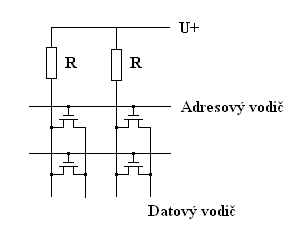
\includegraphics[width=1\linewidth]{EEPROM.png}
\end{multicols}
\subsection{FLASH}
Obdoba EEPROM paměti.
Jsou to paměti statické a elektricky nezávislé.
Programují se přímo v počítači.
Paměti není nutné z počítače pro programování vyjmout.
Zapisuje so do ní po blocích a celá pamět se zapíše v rámci sekund.
Pracuje se s nimi jako s pamětmi RAM, ale po odpojení se jejich obsah nesmaže.
Při použití k uložení BIOSu, tak se BIOS dá aktualizovat.
Existují dva základní typy těchto pamětí, podle použitých logických hradel.
\subsubsection{NOR Flash paměť}

\subsubsection{NAND Flash paměť}
\subsection{SSD}
Paměti, využívané v dnešních počítačích jako nástpuce pevných disků.
Používají se zde paměti typu SRAM či DRAM.
Většinou se pro ně používají rozhraní SATA či PCIe.
Nemají žádné pohyblivé části, což znamená nižší spotřebu.
Mají rychlejší přístup k datům a mají větší přenosové rychlosti.
Podle použitých čipů mají jsou buďto dražší s vyšší životností nebo levnější s kratší životností.
Čipy:
\subsubsection{SLC}
Na každé paměťové buňce je jeden bit.
Výhodou je vyšší rychlost a menší spotřeba.
\subsubsection{MLC}
